\chapter{Projekt systemu}
\author{Filip Czajkowski}
\section{Cele systemu}
\paragraph{}Wytworzony system miał na celu umożliwić wygenerowanie rozkładu zajęć na podstawie dostępnych danych opisujących daną placówkę edukacyjną. Główny wysiłek został położony na implementację algorytmów, które plan układają, natomiast aplikacja webowa miała służyć jako prosty interfejs do ich wywoływania. Poprzez zastosowanie kilku algorytmów do rozwiązania tego problemu, system umożliwiać miał porównanie ich wydajności. Dodatkowo miał także udostępniać wizualną prezentację powstałego planu dla danego programu nauczania, aby móc go ocenić pod kątem praktycznego zastosowania.
\section{Wymagania}
\paragraph{}Powstały system miał narzucone następujące ograniczenia techniczne:
\begin{itemize}
\item Aplikacja po stronie klienta jest dostępna z poziomu przeglądarki z obsługą JavaScript i wymaga jedynie aktywnego połączenia z serwerem.
\item Aby uruchomić algorytmy po stronie serwera, potrzebne jest posiadanie zainstalowanych następujących komponentów:
\begin{enumerate}
\item kompilator języka \emph{Python 2.7}
\item środowisko wytwórcze aplikacji internetowych w języku Python \emph{Django 1.6}
\item system rozproszonego kolejkowania zadań \emph{Celery 3.1}
\item system komunikacji kolejek systemowych \emph{RabbitMQ 3}
\item obsługa bazy danych \emph{SQLite v.3}
\item obsługa biblioteki JavaScript \emph{ExtJS 4.2}
\item obsługa stylów i widoków w języku HTML \emph{Bootstrap 3.0.3}.
\end{enumerate}
\end{itemize}
\paragraph{}Wymagania funkcjonalne:
\begin{itemize}
\item Konieczność logowania się w celu korzystania z systemu.
\item Możliwość wywołania procesu generowania planu zajęć z koniecznością wyboru algorytmu.
\item Możliwość ustawienia limitu czasowego na czas działania procesu.
\item Pobieranie z pliku tekstowego wedle ustalonego wzorca zestawu ograniczeń opisujących potrzeby rozkładu zajęć.
\item Podgląd listy wykonanych wcześniej zadań oraz stanu uruchomionych obecnie procesów.
\item Wybranie z listy zadań konkretnego przypadku i odczytanie informacji o przyporządkowanych zajęciach do poszczególnych kursów.
\item W widoku zakończonego zadania możliwość wybrania z listy programów nauczania dowolnego z nich i przedstawienie wszystkich przydzielonych kursów w formie tabeli.
\item Możliwość zapisania na dysku wygenerowanego zestawu planów do arkuszy w pliku w formacie \emph{.csv}.
\end{itemize}
\section{Zastosowanie}
\paragraph{}Wytworzony system może mieć zastosowanie dwojakie. Pierwsze z nich należy do pola naukowo - badawczego i szczególnie pod tym kątem było projektowane. Dotyczy ono samego zagadnienia układania planu zajęć, umożliwia porównanie zastosowanych trzech metod pod kątem np. czasu pracy czy samej efektywności procesu. Drugim obszarem zastosowań jest platforma biznesowa, choć dość ograniczona w tym przypadku. Posiadając dane na temat jakiejś placówki dydaktycznej w odpowiednim formacie będziemy mogli ułożyć dla niej realny rozkład zajęć. Udostępniany przez system sposób wizualizacji wynikowego planu umożliwia poddanie go trafnej ocenie przydatności przez człowieka.
\subsection{Przypadki użycia}
\begin{itemize}
\item{\textbf{Aktorzy}} - Wszyscy mogą korzystać z systemu w ten sam sposób, więc istnieje jeden aktor, podstawowy użytkownik systemu. Natomiast aby przeprowadzić jakąkolwiek operację konieczne jest zalogowanie się na wcześniej utworzone konto.
\end{itemize}
\paragraph{}Przypadki użycia systemu, pod których kątem zostały zdefiniowane wymagania i wytworzony cały system prezentują się następująco.
\begin{center}
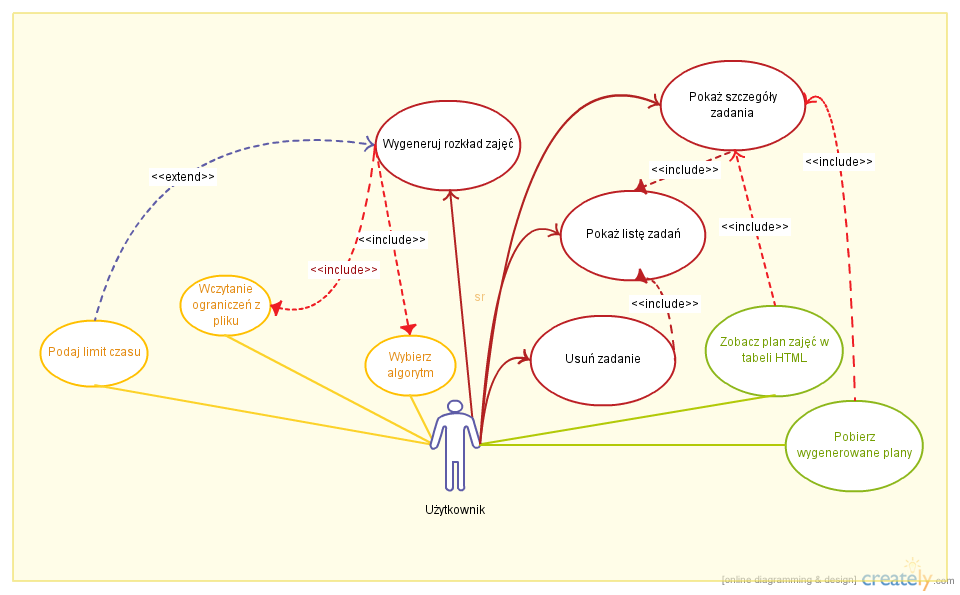
\includegraphics[width=0.8\textwidth]{img/InzynierkaUseCase.png}
\end{center}
\begin{enumerate}
\item{Wygeneruj rozkład zajęć} - Po zalogowaniu z górnego menu wybrać opcję \emph{Add task} i wyświetli się widok umożliwiający wyspecyfikowanie nowego zadania generującego rozkład zajęć.
\item{Podaj limit czasu} - Po wybraniu z menu opcji \emph{Add task} możliwe będzie wpisanie limitu na czas działania algorytmu w sekundach.
\item{Wczytanie ograniczeń z pliku} - Po wybraniu z menu opcji \emph{Add task} widoczny będzie formularz umożliwiający wybór pliku ze zdefiniowanym problemem.
\item{Wybierz algorytm} - Po wybraniu z menu opcji \emph{Add task} w widocznym formularzu dostępna jest lista trzech algorytmów, które będę sterować procesem generacji planu.
\item{Pokaż szczegóły zadania} - Po wybraniu zadania z listy poprzez kliknięcie \emph{Details} ukarze się widok ze szczegółami dotyczącymi konkretnego planu.
\item{Pokaż listę zadań} - Po wybraniu z menu opcji \emph{List all tasks} pokaże się lista dotychczas wykonanych zadań.
\item{Usuń zadanie} - Po wybraniu z menu opcji \emph{List all tasks} pokaże się lista zadań, a każde z nich będzie można usunąć poprzez kliknięcie na przycisk \emph{Delete}, co wywoła następnie odświeżenie listy.
\item{Zobacz plan zajęć w tabeli HTML} - Po wybraniu konkretnego zadania z widoku listy, dla każdego elementu z listy programów nauczania zawartych w planie, dostępny będzie przycisk wywołujący wizualizację wygenerowanego dla niego planu w postaci tabeli HTML.
\item{Pobierz wygenerowane plany} - Po wybraniu konkretnego zadania z widoku listy, dostępny będzie przycisk umożliwiający pobranie wszystkich planów w postaci arkuszy w pliku \emph{.csv}.
\end{enumerate}
\section{Architektura systemu}
\paragraph{} Ogólna architektura systemu oparta jest na modelu klient - serwer. Wszystkie operacje logiczne są wykonywane po stronie serwera, natomiast część kliencka odpowiada jedynie za pobranie danych i prezentację wyników. W części serwera zawarte są następujące komponenty.
\begin{enumerate}
\item Oprogramowanie obsługi serwera wykonane w środowisku \emph{Python}, które generuje widok strony internetowej, odbiera żądania klienta itd.
\item Moduł odpowiedzialny za wyświetlanie planów zajęć na podstawie informacji zawartych w pliku wynikowym algorytmu.
\item Baza danych \emph{SQLite} zawierająca informacje o użytkownikach systemu oraz wykonanych zadaniach.
\item Moduły generujące plany zajęć realizujące poszczególne algorytmy wykonane w technologii \emph{Python}.
\item Komponent \emph{Celery} realizujący zadania z kolejki zadań wywołujący wskazane algorytmy.
\end{enumerate}
\begin{figure}[H]
  \caption{Diagram komponentów systemu}
  \centering
    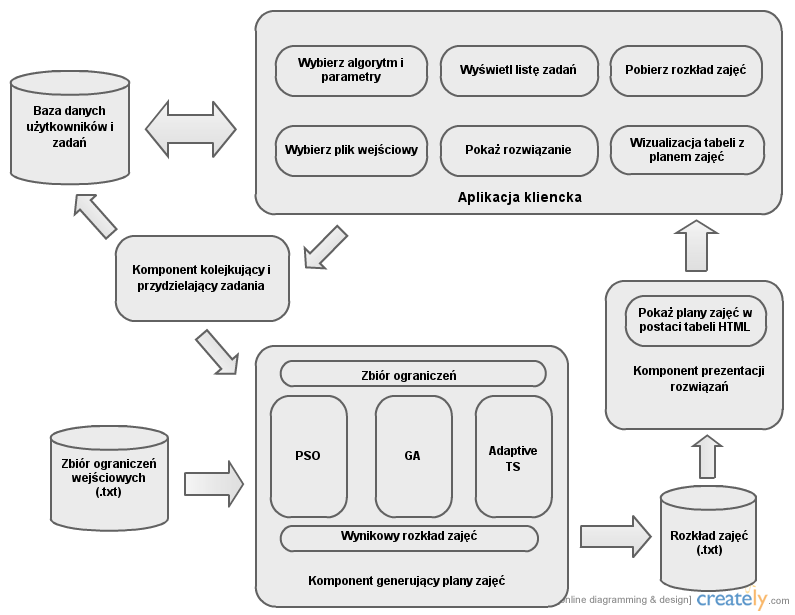
\includegraphics[width=0.8\textwidth]{img/ComponentsDiagram.png}
\end{figure}
\section{Rozwiązania implementacyjne}
\paragraph{Komunikacja} - schemat komunikacji w systemie po stronie serwera podczas wywołania zadania generującego plan prezentuje poniższy diagram.
\begin{figure}[H]
  \caption{Diagram komunikacji po stronie serwera}
  \centering
    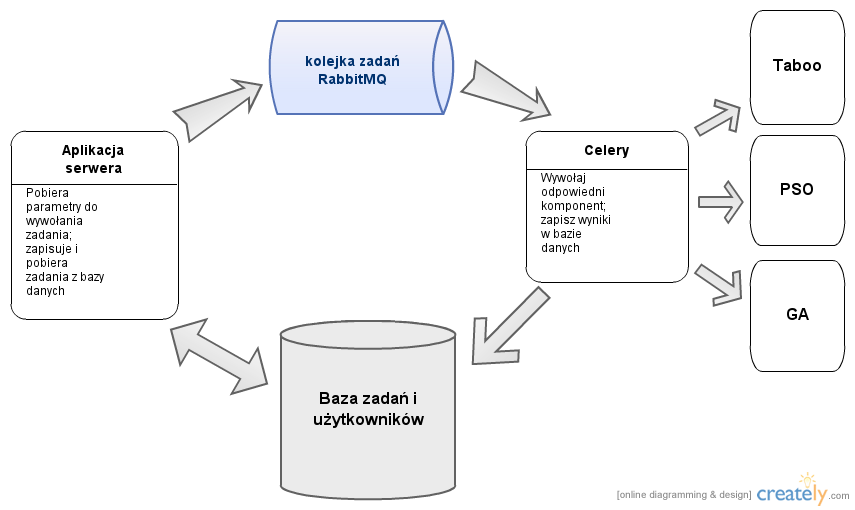
\includegraphics[width=0.8\textwidth]{img/SystemCommunication.png}
\end{figure}
Gdy użytkownik prześle plik wejściowy i parametry wykonania, następuje wywołanie procedury wytworzenia planu zajęć. Aplikacja serwera przekazuje wiadomość o potrzebie wykonania zadania wraz z informacją jaki algorytm wywołać i gdzie znajduje się plik wejściowy. Zlecone zadania są zapamiętywane w kolejce systemowej. Następnie, gdy obiekt wywołujący zadania jest wolny, podbiera z kolejki zadanie i następnie wywołuje odpowiedni komponent wskazany przez typ stosowanego algorytmu. Po wykonaniu zadania zapisuje zwrócony plan zajęć do pliku i dodaje w bazie danych wpis o kolejnym zakończonym zadaniu. Dzięki tej informacji aplikacja kliencka może później pobrać informacje o wygenerowanym planie.
\paragraph{}W celu zapisywania wygenerowanych planów, została stworzona  na serwerze określona struktura plików. Istnieją dwa foldery \emph{input} oraz \emph{output}, w których składowane są pliki odpowiednio z danymi wejściowymi dla algorytmu oraz z planem wynikowym. Rozróżniane są dzięki swojej nazwie, która odpowiada numerowi identyfikującemu zadanie w bazie danych.
\paragraph{} Implementacja samych komponentów generujących plan wedle trzech algorytmów powstawała przy współudziale czterech osób. Stąd współdzielą one część kodu, ale też niektóre stosowane struktury są odmienne. Szczegółowy opis struktur poszczególnych rozwiązań zawiera się w rozdziale Implementacja.